\definecolor{netlgreen}{RGB}{137,190,49}
\definecolor{netlnavy}{RGB}{20,31,46}
\definecolor{netlteal}{RGB}{20,101,116}
\definecolor{netlgray}{RGB}{92,103,112}
\definecolor{netlmist}{RGB}{238,246,242}
\definecolor{netlwarning}{RGB}{175,88,28}

\molochset{
  colors/theme=highcontrast,
  colors/variant=light,
  titleformat section=allcaps,
  progressbar linewidth=1.35pt
}
\setbeamersize{text margin left=8mm,text margin right=8mm}

\setbeamercolor{normal text}{fg=netlnavy,bg=white}
\setbeamercolor{alerted text}{fg=netlteal}
\setbeamercolor{structure}{fg=netlteal}
\setbeamercolor{title}{fg=netlnavy}
\setbeamercolor{subtitle}{fg=netlteal}
\setbeamercolor{frametitle}{fg=netlnavy,bg=white}
\setbeamercolor{progress bar}{fg=netlgreen,bg=netlnavy!12}
\setbeamercolor{title separator}{fg=netlgreen}
\setbeamercolor{block title}{fg=white,bg=netlteal}
\setbeamercolor{block body}{fg=netlnavy,bg=netlmist}
\setbeamercolor{block title alerted}{fg=white,bg=netlwarning}
\setbeamercolor{block body alerted}{fg=netlnavy,bg=netlwarning!8}
\setbeamercolor{block title example}{fg=white,bg=netlgreen!70!netlnavy}
\setbeamercolor{block body example}{fg=netlnavy,bg=netlgreen!10}
\setbeamercolor{standout}{fg=white,bg=netlnavy}
\setbeamercolor{footline}{fg=netlgray,bg=white}
\setbeamercolor{page number in head/foot}{fg=netlgray}

\setbeamerfont{title}{series=\bfseries,size=\LARGE}
\setbeamerfont{subtitle}{size=\large}
\setbeamerfont{frametitle}{series=\bfseries,size=\large}
\setbeamerfont{section title}{series=\bfseries,size=\Large}
\setbeamerfont{block title}{series=\bfseries}
\setbeamerfont{standout}{series=\bfseries,size=\Large}
\setbeamerfont{page number in head/foot}{size=\tiny}

\setbeamertemplate{navigation symbols}{}
\setbeamertemplate{page number in head/foot}[totalframenumber]

\newcommand{\coverprocessmark}{%
  
\begin{tikzpicture}[x=1cm,y=1cm,baseline]
    \draw[netlgreen,line width=1.3pt] (0,0) -- (2.8,0);
    \foreach \x/\lab in {0/Brine,0.95/Pretreat,1.9/$D_i$,2.8/TEA} {
      \fill[netlteal] (\x,0) circle (2.1pt);
      \node[font=\scriptsize,text=netlgray,anchor=north] at (\x,-0.08) {\lab};
    }
  \end{tikzpicture}%
}

\newcommand{\processbridge}[1]{%
  \resizebox{#1\linewidth}{!}{%
    \begin{tikzpicture}[
      node distance=0.25cm,
      box/.style={
        rounded corners=1.8pt,
        draw=netlteal!60,
        fill=netlmist,
        line width=0.45pt,
        align=center,
        minimum width=1.75cm,
        minimum height=0.72cm,
        font=\scriptsize
      },
      arrow/.style={-{Latex[length=2mm]},line width=0.65pt,draw=netlgreen!80!netlnavy}
    ]
      \node[box] (feed) {Smackover\\clean Li/Na};
      \node[box,right=of feed] (reagent) {Rezaee\\DES/TOPO};
      \node[box,right=of reagent] (dist) {$\log D_i$\\surfaces};
      \node[box,right=of dist] (ms) {PrOMMiS\\MSContactor};
      \node[box,right=of ms] (cost) {IDAES\\costing};
      \draw[arrow] (feed) -- (reagent);
      \draw[arrow] (reagent) -- (dist);
      \draw[arrow] (dist) -- (ms);
      \draw[arrow] (ms) -- (cost);
      \node[font=\tiny,text=netlgray,align=center,below=0.12cm of dist] {Transfer variables, validity flags, and costing basis stay traceable};
    \end{tikzpicture}%
  }%
}

\newcommand{\costingplot}{%
  \begin{tikzpicture}
    \begin{axis}[
      width=0.94\linewidth,
      height=0.34\textheight,
      ybar=0pt,
      bar width=9pt,
      ymin=0,
      ymax=16,
      ylabel={\scriptsize USD/year, millions},
      symbolic x coords={Stress,Base,Favorable},
      xtick=data,
      tick label style={font=\scriptsize,text=netlnavy},
      label style={font=\scriptsize,text=netlgray},
      legend style={font=\tiny,draw=none,fill=none,at={(0.02,0.98)},anchor=north west},
      axis line style={netlgray!45},
      ymajorgrids,
      grid style={netlgray!12},
      nodes near coords,
      every node near coord/.append style={font=\tiny,rotate=90,anchor=west,text=netlnavy},
    ]
      \addplot[fill=netlteal!80,draw=netlteal] coordinates {(Stress,1.00) (Base,1.58) (Favorable,2.41)};
      \addplot[fill=netlgreen!85!netlnavy,draw=netlgreen!70!netlnavy] coordinates {(Stress,0.59) (Base,3.67) (Favorable,14.52)};
      \legend{annual cost,net before tax}
    \end{axis}
  \end{tikzpicture}%
}

\newcommand{\validationriskplot}{%
  \begin{tikzpicture}
    \begin{axis}[
      xbar,
      width=0.82\linewidth,
      height=0.43\textheight,
      xmin=0,
      xmax=450,
      xlabel={\scriptsize Na/Li mass ratio},
      symbolic y coords={Rezaee DOE max,MS-2 feed},
      ytick=data,
      tick label style={font=\scriptsize,text=netlnavy},
      label style={font=\scriptsize,text=netlgray},
      axis line style={netlgray!45},
      xmajorgrids,
      grid style={netlgray!12},
      nodes near coords,
      every node near coord/.append style={font=\scriptsize,text=netlnavy},
    ]
      \addplot[fill=netlteal!70,draw=netlteal] coordinates {(15,Rezaee DOE max)};
      \addplot[fill=netlwarning!90,draw=netlwarning] coordinates {(381.5,MS-2 feed)};
    \end{axis}
  \end{tikzpicture}%
}
